\documentclass[../../circle.tex]{subfiles}
\usepackage{tikz}
\usepackage{amsmath}
\usetikzlibrary{calc}

\usetkzlibrary{angles}
\setcounter{secnumdepth}{3} % 让三级标题有编号
\setcounter{tocdepth}{3}    % 目录显示到三级标题
\renewcommand{\thesubsubsection}{\arabic{subsubsection}} 
\begin{document}
\subsubsection{最值问题}

如图,在 $\triangle ABC$ 中,$CA = CB = 5$,$AB = 6$,$D$ 为 $AB$ 边上一动点,连接 $CD$,将 $CD$ 绕点 $C$ 逆时针旋转到 $CE$,使 $\angle ACB = \angle DCE$。连接 $DE$ 交 $BC$ 于点 $F$。则 $CF$ 的最小值为\underline{\quad\quad\quad}。

\vspace{1em}
\begin{center}
    \begin{minipage}{0.45\textwidth}
        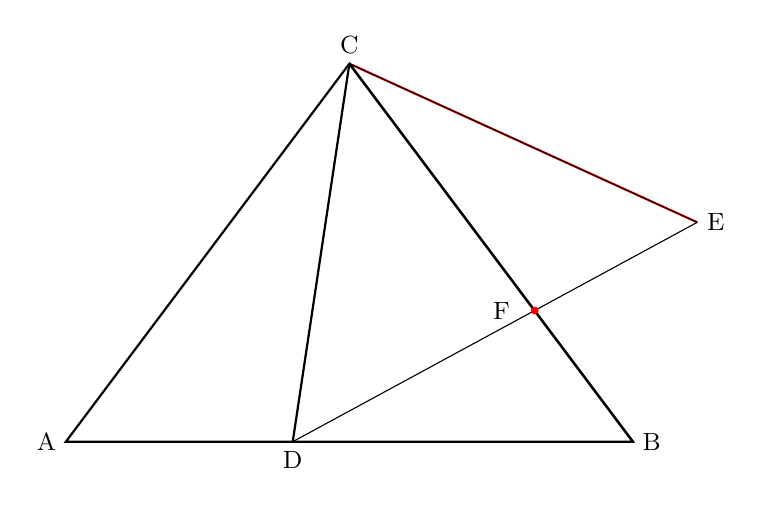
\begin{tikzpicture}[scale=1.2]
            % 三角形ABC构造
            \coordinate (A) at (0,0);
            \coordinate (B) at (6,0);
            \coordinate (C) at (3,4); % 顶点C在上方,构成等腰三角形

            \draw[thick] (A) -- (B) -- (C) -- cycle;
            \node[left] at (A) {\small A};
            \node[right] at (B) {\small B};
            \node[above] at (C) {\small C};

            % 点D在AB边上(可调位置)
            \coordinate (D) at ($(A)!0.4!(B)$);
            \node[below] at (D) {\small D};
            \draw[thick] (C) -- (D);

            % 绕点C逆时针旋转CD得到CE,使∠ACB = ∠DCE
            % 计算CD向量
            % 计算CD向量并旋转
            % \path let \p1 = (C), \p2 = (D) in
            % \pgfextra{
            %     \pgfmathsetmacro{\dx}{\x2 - \x1}
            %     \pgfmathsetmacro{\dy}{\y2 - \y1}
            %     \pgfmathsetmacro{\angleACB}{70}
            %     \pgfmathsetmacro{\cosAngle}{cos(\angleACB)}
            %     \pgfmathsetmacro{\sinAngle}{sin(\angleACB)}
            %     \xdef\ex{\cosAngle*\dx - \sinAngle*\dy}
            %     \xdef\ey{\sinAngle*\dx + \cosAngle*\dy}
            % };
            % \coordinate (E) at ($(C) + (\ex pt, \ey pt)$);
            % \draw[thick,red,rotate around={106:(C)}] (C) -- (D) node[right] {G};

            \pgfmathsetmacro{\angleACB}{74} % 旋转角度
            \path let \p1 = (C), \p2 = (D) in
            coordinate (E) at
            ($(C)+({cos(\angleACB)*(\x2-\x1) - sin(\angleACB)*(\y2-\y1)},
                {sin(\angleACB)*(\x2-\x1) + cos(\angleACB)*(\y2-\y1)})$);
            \draw[thick,red] (C) -- (E);






            \node[right] at (E) {\small E};



            \draw (C) -- (E);

            % 连接DE并与BC交于F
            \draw (D) -- (E);
            \draw[thick] (B) -- (C);
            \coordinate (F) at (intersection of D--E and B--C);
            \filldraw[red] (F) circle (1pt);
            \node[xshift = -12pt] at (F) {\small F};
        \end{tikzpicture}
    \end{minipage}

\end{center}
\textbf{解:}
设 $AD = x$,则 $DB=6-x$,\newline
$\triangle ACD \sim \triangle BDF$,\newline
$\frac{AC}{BD} = \frac{AD}{BF}$,\newline
$\frac{5}{6-x} = \frac{x}{BF}$,\newline
$BF = \frac{6x-x^2}{5}$,\newline
$BF$最大值为 $\frac{9}{5}$。\newline
$\therefore \min CF = \frac{16}{5}$。
\begin{tcolorbox}[colback=blue!5!white,colframe=blue!75!black,title=提示]
    最值问题,以前都是靠两点之间线段最短、垂线段最短,这里是靠方程来解决。这也是一个很好的方法。
\end{tcolorbox}
\subsubsection{比相关}
如图,在三角形 $\triangle ABC$ 中,$AB = AC$,$\angle B = 30^\circ$,点 $D$、$E$ 是边 $BC$ 上的两个动点,且满足 $\angle DAB = 60^\circ$。若以 $BD$、$DE$、$EC$ 的长度为边长构成一个直角三角形,则 $BD : EC$ 的可能值是:
\begin{center}


    \begin{tasks}(4) % 括号内数字表示每行最多几个选项
        \task[A.] $2 : 1$
        \task[B.] $\sqrt{3} : 1$
        \task[C.] $\sqrt{3} : 2$
        \task[D.] $2 : \sqrt{3}$
    \end{tasks}
\end{center}

\begin{center}
    \begin{minipage}{0.45\textwidth}
        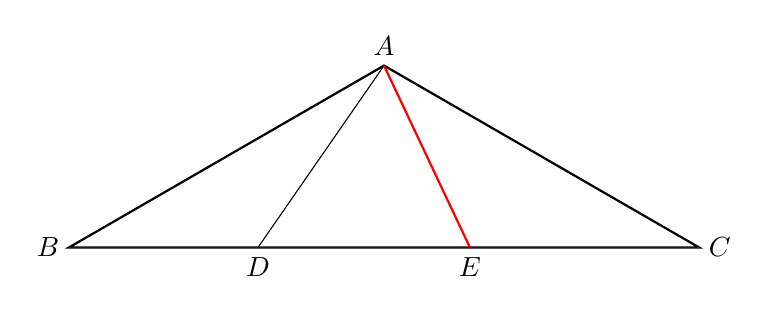
\begin{tikzpicture}[scale=1]
            % 定义点
            \coordinate (B) at (0,0);
            \coordinate (C) at (8,0);
            \coordinate (A) at (4,2.309); % AB = AC, ∠B = 30°, 所以 AB = AC = 4, 高 = 4*sin(60°) ≈ 3.464

            % 边界三角形
            \draw[thick] (A) -- (B) -- (C) -- cycle;

            % 标注点
            \node[left] at (B) {$B$};
            \node[right] at (C) {$C$};
            \node[above] at (A) {$A$};

            % 点 D 和 E 在 BC 上
            \coordinate (D) at ($(B)!0.3!(C)$);

            \draw (A) -- (D);


            % 标注 D 和 E
            \node[below] at (D) {$D$};
            \pgfmathsetmacro{\angleACB}{60} % 旋转角度
            \path let \p1 = (A), \p2 = (D) in
            coordinate (E2) at
            ($(A)+({cos(\angleACB)*(\x2-\x1) - sin(\angleACB)*(\y2-\y1)},
                {sin(\angleACB)*(\x2-\x1) + cos(\angleACB)*(\y2-\y1)})$);
            \coordinate (E) at (intersection of C--B and A-- E2);
            \draw[thick,red] (A) -- (E);
            \node[below] at (E) {$E$};

            % 辅助线 BD, DE, EC
            \draw[blue] (B) -- (D);
            \draw[blue] (D) -- (E);
            \draw[blue] (E) -- (C);
            % 自动测量并显示角度 ∠AOB
            % 计算角度并存储
            % \tkzGetAngle(E,A,C){ang} % ang 是变量名
            % 显示角度数值
            %   \tkzLabelAngle[pos=0.8](A,O,B){\ang$^\circ$}
            % \tkzLabelAngle[pos=0.8](E,A,C){$\tkzGetAngle$}; % 自动显示角度数值



        \end{tikzpicture}
    \end{minipage}


\end{center}

\textbf{解:}
这里需要把这三条线段组成一个首尾相接的三角形。
把$\triangle ABD$进行旋转$120^\circ$,得到$\triangle AD'C$。\
期中$\angle ACD=30^\circ$,所以$\angle D'CE=60^\circ$。$\triangle ADE \simeq \triangle AED'$,所以$DE=D'E$。
此时三条边终于到了一个直角三角形。D与E的位置决定
\begin{center}

    \begin{minipage}{0.45\textwidth}
        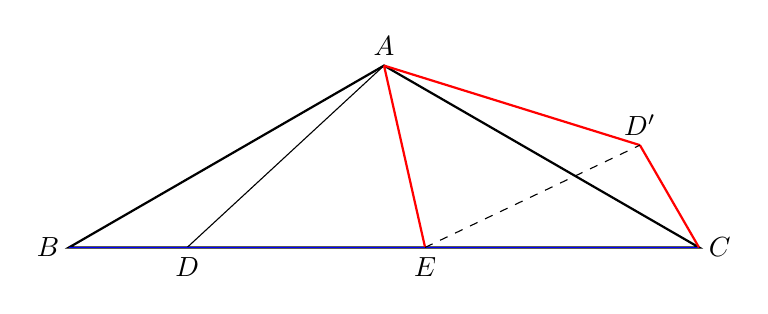
\begin{tikzpicture}[scale=1]
            % 定义点
            \coordinate (B) at (0,0);
            \coordinate (C) at (8,0);
            \coordinate (A) at (4,2.3094); % AB = AC, ∠B = 30°, 所以 AB = AC = 4, 高 = 4*sin(60°) ≈ 3.464

            % 边界三角形
            \draw[thick] (A) -- (B) -- (C) -- cycle;

            % 标注点
            \node[left] at (B) {$B$};
            \node[right] at (C) {$C$};
            \node[above] at (A) {$A$};

            % 点 D 和 E 在 BC 上
            \coordinate (D) at (1.5,0);

            \draw (A) -- (D);


            % 标注 D 和 E
            \node[below] at (D) {$D$};
            \pgfmathsetmacro{\angleACB}{60} % 旋转角度
            \path let \p1 = (A), \p2 = (D) in
            coordinate (E2) at
            ($(A)+({cos(\angleACB)*(\x2-\x1) - sin(\angleACB)*(\y2-\y1)},
                {sin(\angleACB)*(\x2-\x1) + cos(\angleACB)*(\y2-\y1)})$);
            \coordinate (E) at (intersection of C--B and A-- E2);
            \draw[thick,red] (A) -- (E);
            \node[below] at (E) {$E$};

            % 辅助线 BD, DE, EC
            \draw[blue] (B) -- (D);
            \draw[blue] (D) -- (E);
            \draw[blue] (E) -- (C);
            % \path let \p1 = (E) in
            % node at (2,2) {x=\x1, y=\y1};
            % 相对坐标:A-B
            % 相对坐标:A-B
            % \coordinate (G) at ($(A)-(B)$); % 得到 A-B 的相对坐标
            % \path let \p1 = (G) in
            % node at (2,2) {x=\x1, y=\y1};
            % \node at (0,0) {x=\x1,y=\y1};
            % 提取x和y坐标
            % 定义点
            % \coordinate (P) at (1.5,2.5);

            % 提取x和y坐标

            %         \path let \p1 = (P) in
            %   \pgfextra{
            %     \pgfmathsetmacro{\myx}{\x1}
            %     \pgfmathsetmacro{\myy}{\y1}
            %   }
            %   node at (3,1) {Point P coord: (\myx, \myy)};



            \pgfmathsetmacro{\angleACB}{120} % 旋转角度
            \path let \p1 = (A), \p2 = (D) in
            coordinate (D') at
            ($(A)+({cos(\angleACB)*(\x2-\x1) - sin(\angleACB)*(\y2-\y1)},
                {sin(\angleACB)*(\x2-\x1) + cos(\angleACB)*(\y2-\y1)})$);
            \draw[thick,red] (A) -- (D');
            \draw[thick,red] (C) -- (D');
            \draw[dashed] (E) -- (D');
            \node[above] at (D') {$D'$};



        \end{tikzpicture}
    \end{minipage}
\end{center}
\begin{center}
 \begin{minipage}{0.45\textwidth}
        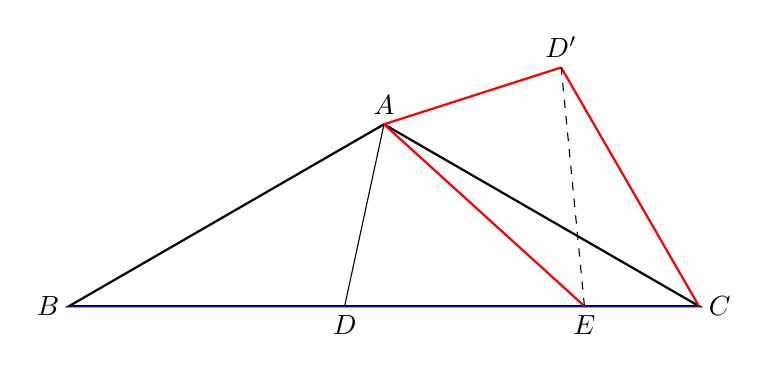
\begin{tikzpicture}[scale=1]
            % 定义点
            \coordinate (B) at (0,0);
            \coordinate (C) at (8,0);
            \coordinate (A) at (4,2.3094); % AB = AC, ∠B = 30°, 所以 AB = AC = 4, 高 = 4*sin(60°) ≈ 3.464

            % 边界三角形
            \draw[thick] (A) -- (B) -- (C) -- cycle;

            % 标注点
            \node[left] at (B) {$B$};
            \node[right] at (C) {$C$};
            \node[above] at (A) {$A$};

            % 点 D 和 E 在 BC 上
            \coordinate (D) at (3.5,0);

            \draw (A) -- (D);


            % 标注 D 和 E
            \node[below] at (D) {$D$};
            \pgfmathsetmacro{\angleACB}{60} % 旋转角度
            \path let \p1 = (A), \p2 = (D) in
            coordinate (E2) at
            ($(A)+({cos(\angleACB)*(\x2-\x1) - sin(\angleACB)*(\y2-\y1)},
                {sin(\angleACB)*(\x2-\x1) + cos(\angleACB)*(\y2-\y1)})$);
            \coordinate (E) at (intersection of C--B and A-- E2);
            \draw[thick,red] (A) -- (E);
            \node[below] at (E) {$E$};

            % 辅助线 BD, DE, EC
            \draw[blue] (B) -- (D);
            \draw[blue] (D) -- (E);
            \draw[blue] (E) -- (C);
            % \path let \p1 = (E) in
            % node at (2,2) {x=\x1, y=\y1};
            % 相对坐标:A-B
            % 相对坐标:A-B
            % \coordinate (G) at ($(A)-(B)$); % 得到 A-B 的相对坐标
            % \path let \p1 = (G) in
            % node at (2,2) {x=\x1, y=\y1};
            % \node at (0,0) {x=\x1,y=\y1};
            % 提取x和y坐标
            % 定义点
            % \coordinate (P) at (1.5,2.5);

            % 提取x和y坐标

            %         \path let \p1 = (P) in
            %   \pgfextra{
            %     \pgfmathsetmacro{\myx}{\x1}
            %     \pgfmathsetmacro{\myy}{\y1}
            %   }
            %   node at (3,1) {Point P coord: (\myx, \myy)};



            \pgfmathsetmacro{\angleACB}{120} % 旋转角度
            \path let \p1 = (A), \p2 = (D) in
            coordinate (D') at
            ($(A)+({cos(\angleACB)*(\x2-\x1) - sin(\angleACB)*(\y2-\y1)},
                {sin(\angleACB)*(\x2-\x1) + cos(\angleACB)*(\y2-\y1)})$);
            \draw[thick,red] (A) -- (D');
            \draw[thick,red] (C) -- (D');
            \draw[dashed] (E) -- (D');
            \node[above] at (D') {$D'$};



        \end{tikzpicture}
    \end{minipage}
  
\end{center}
\begin{tcolorbox}[colback=blue!5!white,colframe=blue!75!black,title=提示]
    这里也可以理解成二倍角模型,与正方形中半角,两个全等相似
\end{tcolorbox}
\subsubsection{求度数}

 
   如图,$\triangle ABC$ 中,$AB = AC$,点 $D, E$ 分别为线段 $BC, AD$ 上的点,$\angle ADC = 60^\circ$,连接 $BE, CE$,已知 $AE = BE$。
  
  \begin{enumerate}
    \item 若 $\angle BAC = 90^\circ$,则 $\angle DCE = \boxed{15^\circ}$。
    \item 若 $\angle BAC = 96^\circ$,则 $\angle DCE = \boxed{12^\circ}$。
  \end{enumerate}
  
  % 图形占位
  \begin{center}
    \begin{tikzpicture}[scale=1]
      % 基本三角形 ABC
      \coordinate (B) at (0,0);
      \coordinate (A) at (3,3.217);
      \coordinate (C) at (6,0);
      \draw (A) -- (B) -- (C) -- cycle;
      \node at (A) [above] {$A$};
      \node at (B) [left] {$B$};
      \node at (C) [ right] {$C$};

     
    \end{tikzpicture}
  \end{center}
 

\end{document}